\section{Experiment C: does an in-context controller explore?}\label{sec:expc}

\begin{figure}[t]
\centering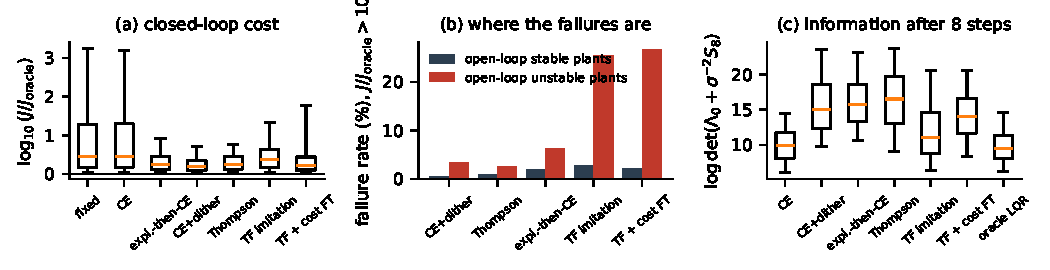
\includegraphics[width=\linewidth]{figs/fig_c.pdf}
\vspace{-6mm}
\caption{\textbf{C} (4096 paired test plants, 3 seeds). (a)~Normalised cost $J/J_{\rm oracle}$; boxes span the 5--95\%
range. Certainty equivalence without excitation never moves $u$, so it learns nothing (Prop.~\ref{prop:ident}).
(b)~Failure rate on open-loop stable vs.\ unstable plants. (c)~Information gathered in the first 8 steps.}
\label{fig:c}
\vspace{-3mm}
\end{figure}

\paragraph{The dual effect in the baselines.} With the prior mean $B{=}0$, certainty equivalence (CE) computes a zero
gain, outputs $u\equiv0$, and so never learns $B$. Its information after 8 steps stays at the prior level
(\CCEinfo\ nats, against \CORCinfo\ for the oracle, which needs none), it fails on \CCEfail\% of plants, and its median cost
is \CCEmed. A constant gain cannot help when the actuation direction is unknown (median \CFIXmed). Any excitation
fixes this: decaying dither (median \CCEDmed, \CCEDfail\% failures, \CCEDinfo\ nats), explore-then-commit (\CETCmed,
\CETCfail\%, \CETCinfo) and Thompson sampling (\CTSmed, \CTSfail\%, \CTSinfo).

\paragraph{The transformer explores, without being told to.} Pre-registered pure BPTT did not train (Appendix,
Table~\ref{tab:pilots}); the controller is a DAgger warm start followed by cost fine-tuning. After the warm start it
gathers \CBCinfo\ nats; cost fine-tuning adds \CinfoFtBc\ \CinfoFtBcci\ more, to \CTFinfo. That is \Hfived\
\Hfivedci\ above CE (H5d, Holm $p\PHfived$). So a controller with no identification objective learns to excite the
plant, and most of that excitation is learned from the cost, not copied from the LQR teacher. It still excites less
than dither (\CinfoCED\ \CinfoCEDci) and Thompson sampling (\CinfoTS\ \CinfoTSci).

\paragraph{Cost: competitive in the typical case, unsafe in the tail.} The median normalised cost is \CTFmed\ (seeds
\CTFmedRange), against \CCEDmed\ for dither and \CTSmed\ for Thompson sampling; per plant, the transformer wins against
Thompson sampling \CwinsTS\% of the time and against dither \CwinsCED\% (paired median differences \CvsTSmed\ \CvsTSmedci\ and
\CvsCEDmed\ \CvsCEDmedci). But it fails on \CTFfail\% of plants against \CCEDfail\%. The failures sit almost
entirely on the \CfracUnst\% of plants that are open-loop unstable: \CfailUnstTF\% there against \CfailStabTF\% on stable
plants (dither: \CfailUnstCED\% and \CfailStabCED\%), Fig.~\ref{fig:c}b. Controllability is not the issue. Because the
mean is dominated by these failures, the transformer beats the constant gain (H5a, Holm $p\PHfivea$) but \emph{not} CE on
the pre-registered mean (H5b: \Hfiveb\ \Hfivebci, $p\PHfiveb$), and it is far worse than every excited baseline in the mean
(vs.\ dither: \CvsCED\ \CvsCEDci).

\paragraph{What cost fine-tuning buys, and what it costs.} Relative to the warm start, fine-tuning on
$\log(J/J_{\rm oracle})$ improves the median (\CBCmed\ to \CTFmed) and the excitation, leaves the failure rate
unchanged (\CBCfail\% to \CTFfail\%) and makes the failures more severe (mean \CBCmean\ to \CTFmean, difference
\CbcMinusFt\ \CbcMinusFtci): the log objective compresses the tail. \PENDING{cvarC}

\paragraph{Exploratory: what the controller identifies, and where.} On its own closed-loop trajectories, the
controller's feedback Jacobian $-\partial u_t/\partial x_t$, its functional gain, approaches the oracle LQR gain as the
context grows ($R^2{=}\CmechGainEnd$ at $t{=}47$), but it extracts less from its data than a classical estimator would:
the certainty-equivalent gain computed from the \emph{same} history is \CmechCEErrEnd\ from the oracle gain in squared
error, against \CmechGainErrEnd\ for the transformer. The actuation matrix $B$ is readable from the key--value fast
weights with $R^2{=}\CmechBfwEarly$ already at $t{=}8$ (\CmechBfwEnd\ at $t{=}47$), against \CmechBresEarly\ (\CmechBresEnd)
from the residual stream at the query position, with the dimension caveat of Appendix~\ref{app:controls}. As in
\S\ref{sec:expa}, the residual-probe directions are inert: flipping the probed estimate flips the action in \Cflip\% of
cases.
